\chapter{Introduction to linear regression}
\label{linRegrForTwoVar}

Linear regression is a very powerful statistical technique. Many people have some familiarity with regression just from reading the news, where graphs with straight lines are overlaid on scatterplots. Linear models can be used for prediction or to evaluate whether there is a linear relationship between two numerical variables.

Figure~\ref{perfLinearModel} shows two variables whose relationship can be modeled perfectly with a straight line. The equation for the line is
\begin{eqnarray*}
y = 7 + 49.24x
\end{eqnarray*}
Imagine what a perfect linear relationship would mean: you would know the exact value of $y$, just by knowing the value of $x$. This is unrealistic in almost any natural process. Consider height and weight of school children for example. Their height, $x$, gives you some information about their weight, $y$, but there is still a lot of variability, even for children of the same height. 
\begin{figure}
   \centering
   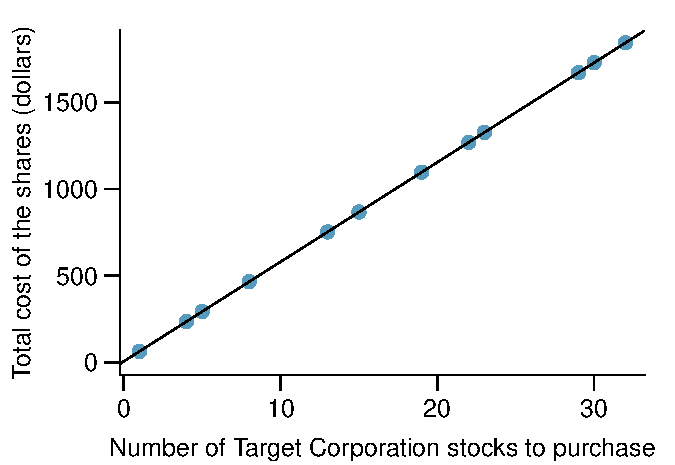
\includegraphics[width=0.6\textwidth]{07/figures/perfLinearModel/perfLinearModel}
   \caption{Twelve requests were put into a trading company to buy Target Corporation stock (ticker \texttt{TGT}, May 24th, 2011), and the total cost of the shares were reported. Because the cost is computed using a linear formula, the linear fit is perfect.}
   \label{perfLinearModel}
\end{figure}

We often write a linear regression line as
\begin{eqnarray*}
y = \beta_0 + \beta_1x
\end{eqnarray*}
\marginpar[\raggedright\vspace{-10mm}

$\beta_0, \beta_1$\\\footnotesize Linear model\\ parameters]{\raggedright\vspace{-10mm}

$\beta_0, \beta_1$\\\footnotesize Linear model\\ parameters}where $\beta_0$ and $\beta_1$ represent two parameters that we wish to identify. Usually $x$ represents an explanatory or \term{predictor} variable and $y$ represents a response. We use the variable $x$ to predict a response $y$. Usually, we use $b_0$ and $b_1$ to denote the point estimates of $\beta_0$ and $\beta_1$.

Examples of several scatterplots are shown in Figure~\ref{imperfLinearModel}. While none reflect a perfect linear relationship, it will be useful to fit approximate linear relationships to each. The lines represent models relating $x$ to $y$. The first plot shows a relatively strong downward linear trend. The second shows an upward trend that, while evident, is not as strong as the first. The last plot shows a very weak downward trend in the data, so slight we can hardly notice it.
\begin{figure}
   \centering
   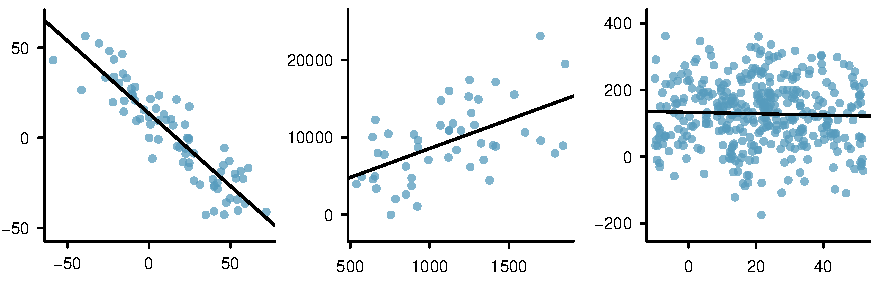
\includegraphics[width=\textwidth]{07/figures/imperfLinearModel/imperfLinearModel}
   \caption{Three data sets where a linear model may be useful but is not perfect.}
   \label{imperfLinearModel}
\end{figure}

We will soon find that there are cases where fitting a straight line to the data, even if there is a clear relationship between the variables, is not helpful. One such case is shown in Figure~\ref{notGoodAtAllForALinearModel} where there is a very strong relationship between the variables even if the trend is not linear. Such nonlinear trends are beyond the scope of this textbook.
\begin{figure}
   \centering
   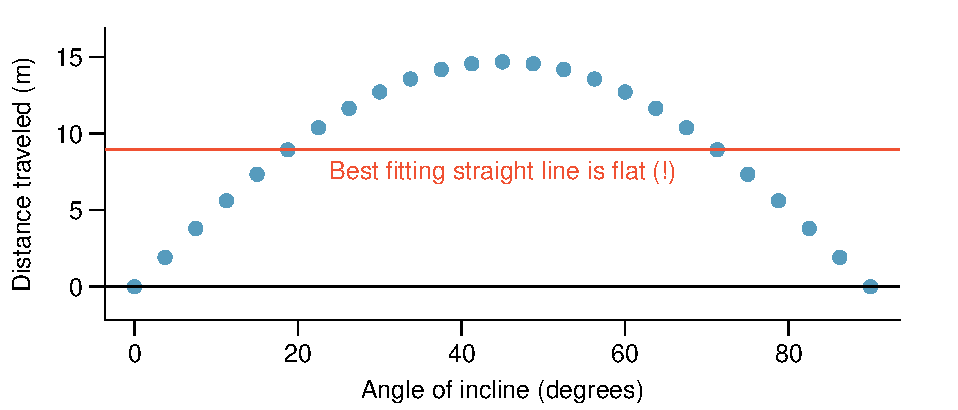
\includegraphics[width=115mm]{07/figures/notGoodAtAllForALinearModel/notGoodAtAllForALinearModel}
   \caption{A linear model is not useful in this nonlinear case. (These data are from an introductory physics experiment.)}
   \label{notGoodAtAllForALinearModel}
\end{figure}


%%%%%%%%%%
\section{Line fitting, residuals, and correlation}
\label{lineFittingResidualsCorrelation}

It is helpful to think deeply about the line fitting process. In this section, we examine criteria for identifying a linear model and introduce a new statistic, \emph{correlation}.

\subsection{Beginning with straight lines}

Scatterplots were introduced in Chapter~\ref{introductionToData} as a graphical technique to present two numerical variables simultaneously. Such plots permit the relationship between the variables to be examined with ease. Figure~\ref{scattHeadLTotalL} shows a scatterplot for the \var{headL} and \var{totalL} variables from the \data{possum} data set introduced in Chapter~\ref{introductionToData}. Each point represents a single possum from the data.
\begin{figure}
   \centering
   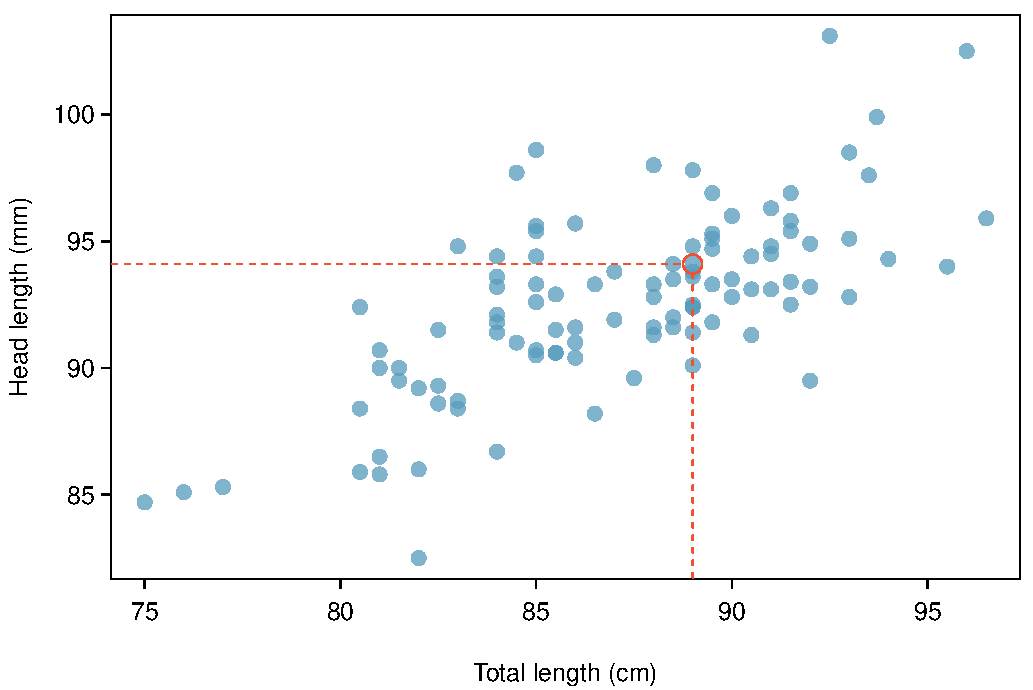
\includegraphics[width=0.79\textwidth]{07/figures/scattHeadLTotalL/scattHeadLTotalL}
   \caption{A scatterplot showing \var{headL} against \var{totalL}. The first possum with a head length of 94.1mm and a length of 89cm is highlighted.}
   \label{scattHeadLTotalL}
\end{figure}

The \var{headL} and \var{totalL} variables are associated. Possums with an above average total length also tend to have above average head lengths. While the relationship is not perfectly linear, it could be helpful to partially explain the connection between these variables with a straight line.
\begin{figure}
   \centering
   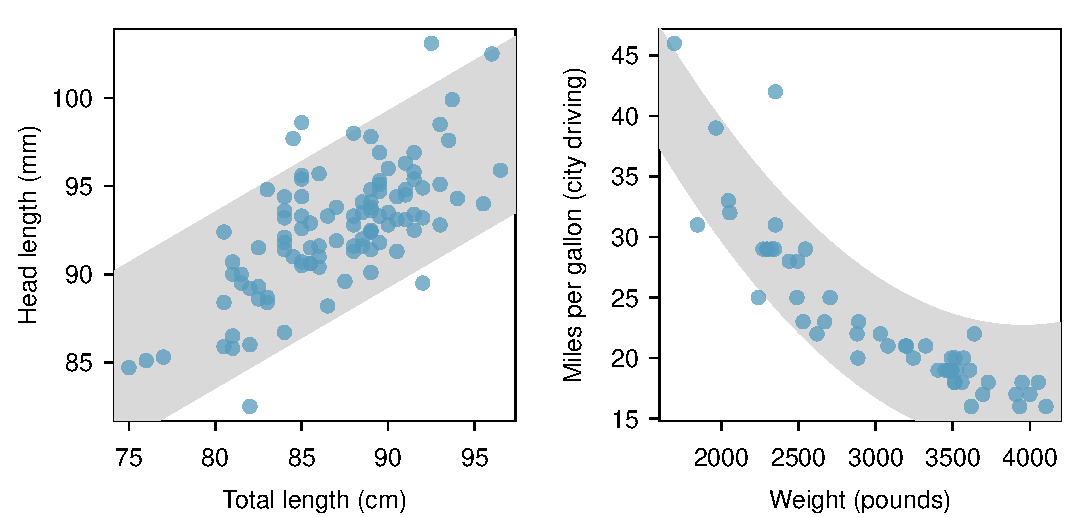
\includegraphics[width=\textwidth]{07/figures/scattHeadLTotalLTube/scattHeadLTotalLTube}
   \caption{Most observations on the left can be captured in a straight band. On the right, we have the \var{weight} and \var{mpgCity} variables represented from the \data{cars} data set, and a curved band does a better job of capturing these cases than a straight band.}
   \label{scattHeadLTotalLTube}
\end{figure}

Straight lines should only be used when the data appear to have a linear relationship, such as the case shown in the left panel of Figure~\ref{scattHeadLTotalLTube}. The right panel of Figure~\ref{scattHeadLTotalLTube} shows a case where a curved band would be more useful in capturing a different set of data.

\begin{caution}
{Watch out for curved trends}
{We only consider models based on straight lines in this chapter. If data show a nonlinear trend, like that in the right panel of Figure~\ref{scattHeadLTotalLTube}, more advanced techniques should be used.}
\end{caution}

\subsection{Fitting a line by eye}

We want to describe the relationship between the \var{headL} and \var{totalL} variables using a line. In this example, we will use the total length as the predictor variable, $x$, to predict a possum's head length, $y$. We could fit the linear relationship by eye, as in Figure~\ref{scattHeadLTotalLLine}. The equation for this line is
\begin{eqnarray}
\widehat{y} = 41 + 0.59*x
\label{headLLinModTotalL}
\end{eqnarray}
We can use this model to discuss properties of possums. For instance, our model predicts a possum with a total length of 80 cm will have a head length of
\begin{eqnarray*}
\widehat{y} = 41 + 0.59*80 = 88.2 mm
\end{eqnarray*}
A ``hat'' on $y$ is used to signify that this is an estimate. The model predicts that possums with a total length of 80 cm will have an average head length of 88.2 mm. Without further information about an 80 cm possum, this prediction for head length that uses the average is a reasonable estimate. Generally, linear models predict the average value of $y$ for a particular value of $x$ based on the model.
\begin{figure}
   \centering
   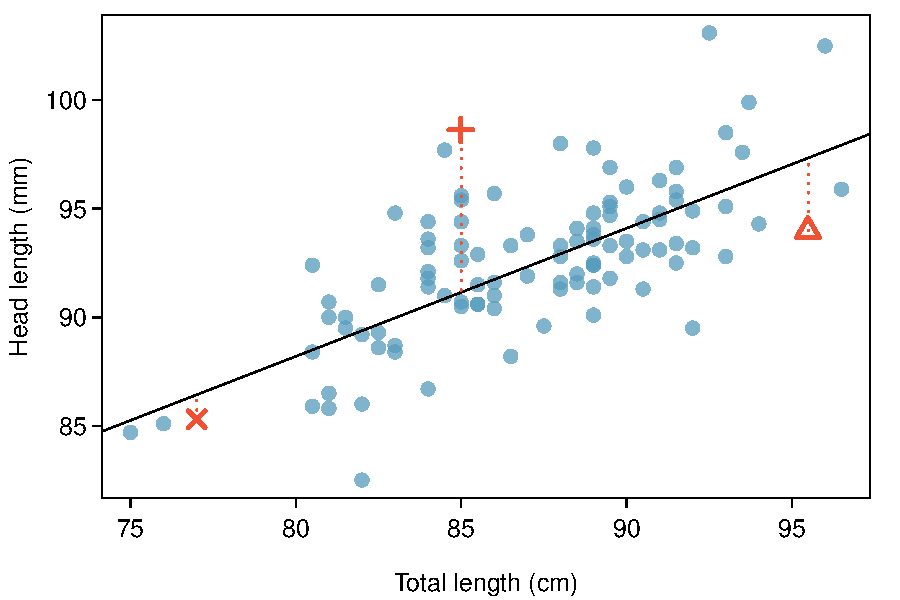
\includegraphics[width=0.85\textwidth]{07/figures/scattHeadLTotalLLine/scattHeadLTotalLLine}
   \caption{A reasonable linear model was fit to represent the relationship between \var{headL} and \var{totalL}.}
   \label{scattHeadLTotalLLine}
\end{figure}

\subsection{Residuals}

\termsub{Residuals}{residuals} can be thought of as the leftovers from the model fit:
\begin{align*}
\text{Data} = \text{Fit} + \text{Residual}
\end{align*}
Each observation will have a residual. If an observation is above the regression line, then its residual, the vertical distance from the observation to the line, is positive. Observations below the line have negative residuals. One goal in picking the right linear model is for these residuals to be as small as possible.

Three observations are noted specially in Figure~\ref{scattHeadLTotalLLine}. The ``$\times$'' has a small, negative residual of about -1; the observation marked by ``$+$'' has a large residual of about +7; and the observation marked by ``$\triangle$'' has a moderate residual of about -4. The size of residuals is usually discussed in terms of its absolute value. For example, the residual for ``$\triangle$'' is larger than that of ``$\times$'' because $|-4|$ is larger than $|-1|$.

\begin{termBox}{\tBoxTitle{Residual: difference between observed and expected}
The \emph{residual} of an observation $(x_i, y_i)$ is the difference of the observed response ($y_i$) and the response we would predict based on the model fit ($\hat{y}_i$):
\begin{eqnarray*}
e_i = y_i - \hat{y}_i
\end{eqnarray*}
We typically identify $\hat{y}_i$ by plugging $x_i$ into the model. The residual of the $i^{th}$ observation is denoted by $e_i$.}
\end{termBox}

\begin{example}{The linear fit shown in Figure~\ref{scattHeadLTotalLLine} is given in Equation~\eqref{headLLinModTotalL}. Based on this line, formally compute the residual of the observation $(77.0, 85.3)$. This observation is denoted by ``$\times$'' on the plot. Check it against the earlier visual estimate, -1.}
We first compute the predicted value of point ``$\times$'' based on the model:
\begin{eqnarray*}
\hat{y}_{\times} = 41+0.59*x_{\times} = 41+0.59*77.0 = 86.4
\end{eqnarray*}
Next we compute the difference of the actual head length and the predicted head length:
\begin{eqnarray*}
e_{\times} = y_{\times} - \hat{y}_{\times} = 85.3 -  86.43 = -0.93
\end{eqnarray*}
This is very close to the visual estimate of -1.
\end{example}

\begin{exercise}
If a model underestimates an observation, will the residual be positive or negative? What about if it overestimates the observation? Answer in the footnote\footnote{If a model underestimates an observation, then the model estimate is below the actual. The residual -- the actual minus the model estimate -- must then be positive. The opposite is true when the model overestimates the observation: the residual is negative.}.
\end{exercise}

\begin{exercise}
Compute the residuals for the observations $(85.0, 98.6)$ (``$+$'' in the figure) and $(95.5, 94.0)$ (``$\triangle$'') using the linear model given in Equation~\eqref{headLLinModTotalL}. Answer for ``$+$'' is in the footnote\footnote{First compute the predicted value based on the model: $$\hat{y}_{+} = 41+0.59*x_{+} = 41+0.59*85.0 = 91.15$$ Then the residual is given by $$e_{+} = y_{+} - \hat{y}_{+} = 98.6-91.15=7.45$$This was close to the earlier estimate of 7.}.
\end{exercise}

Residuals are helpful in evaluating how well a linear model fits a data set. We often display them in a \term{residual plot} such as the one shown in Figure~\ref{scattHeadLTotalLResidualPlot} for the regression line in Figure~\ref{scattHeadLTotalLLine}. The residuals are plotted at their original horizontal locations but with the vertical coordinate as the residual. For instance, the point $(85.0,98.6)_{+}$ had a residual of 7.45, so in the residual plot it is placed at $(85.0, 7.45)$. Creating a residual plot is sort of like tipping the scatterplot over so the regression line is horizontal. 
\begin{figure}
   \centering
   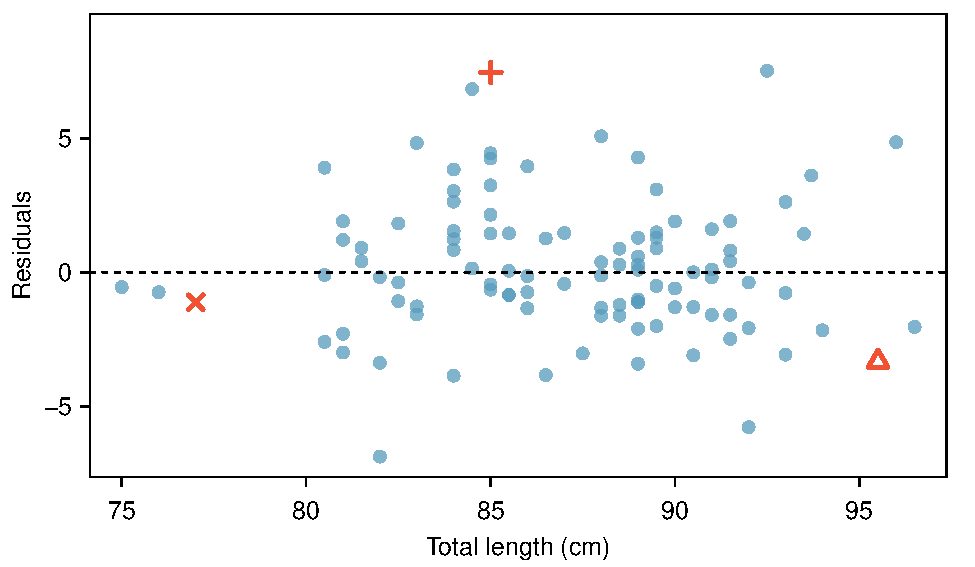
\includegraphics[width=0.85\textwidth]{07/figures/scattHeadLTotalLResidualPlot/scattHeadLTotalLResidualPlot}
   \caption{Residual plot for the model in Figure~\ref{scattHeadLTotalLLine}.}
   \label{scattHeadLTotalLResidualPlot}
\end{figure}

\begin{example}{One purpose of residual plots is to identify characteristics or patterns still apparent in data after fitting a model. Figure~\ref{sampleLinesAndResPlots} shows three scatterplots with linear models in the first row and residual plots in the second row. Can you identify any patterns remaining in the residuals?}
\begin{figure}
   \centering
   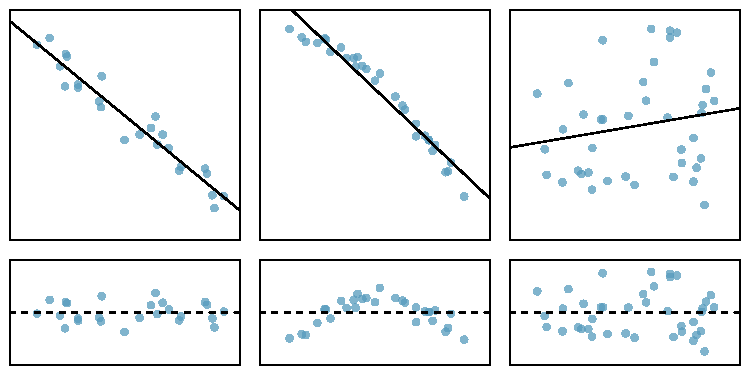
\includegraphics[width=0.8\textwidth]{07/figures/sampleLinesAndResPlots/sampleLinesAndResPlots}
   \caption{Sample data with their best fitting lines (top row) and their corresponding residual plots (bottom row).}
   \label{sampleLinesAndResPlots}
\end{figure}
In the first data set (first column), the residuals show no obvious patterns. The residuals appear to be scattered randomly about 0, represented by the dashed line.

The second data set shows a pattern in the residuals. There is some curvature in the scatterplot, which is more obvious in the residual plot. We should not use a straight line to model these data and should use a more advanced technique instead.

The last plot shows very little upwards trend, and the residuals also show no obvious patterns. It is reasonable to try to fit this linear model to the data. However, it is unclear whether there is statistically significant evidence that the slope parameter is different from zero. The point estimate, $b_1$, is not zero, but we wonder if this could just be due to chance. We will address this sort of question in Section~\ref{inferenceForLinearRegression}.
\end{example}

\subsection{Describing linear relationships with correlation}

\begin{termBox}{\tBoxTitle{Correlation: strength of a linear relationship}
The \term{correlation} describes the strength of the linear relationship between two variables and takes values between -1 and 1. We denote the correlation by $R$.}
\end{termBox}\marginpar[\raggedright\vspace{-11.5mm}

$R$\\\footnotesize correlation]{\raggedright\vspace{-11.5mm}

$R$\\\footnotesize correlation}

We compute the correlation using a formula, just as we did with the sample mean and standard deviation. However, this formula is rather complex\footnote{Formally, we can compute the correlation for observations $(x_1, y_1)$, $(x_2, y_2)$, ..., $(x_n, y_n)$ using the formula
\begin{eqnarray*}
R = \frac{1}{n-1}\sum_{i=1}^{n} \frac{x_i-\bar{x}}{s_x}\frac{y_i-\bar{y}}{s_y}
\end{eqnarray*}
where $\bar{x}$, $\bar{y}$, $s_x$, and $s_y$ are the sample means and standard deviations for each variable.}, so we generally perform the calculations on a computer or calculator. Figure~\ref{posNegCorPlots} shows eight plots and their corresponding correlations. Only when the relationship is perfectly linear is the correlation either -1 or 1. If the relationship is strong and positive, the correlation will be near +1. If it is strong and negative, it will be near -1. If there is no apparent linear relationship between the variables, then the correlation will be near zero.
\begin{figure}
   \centering
   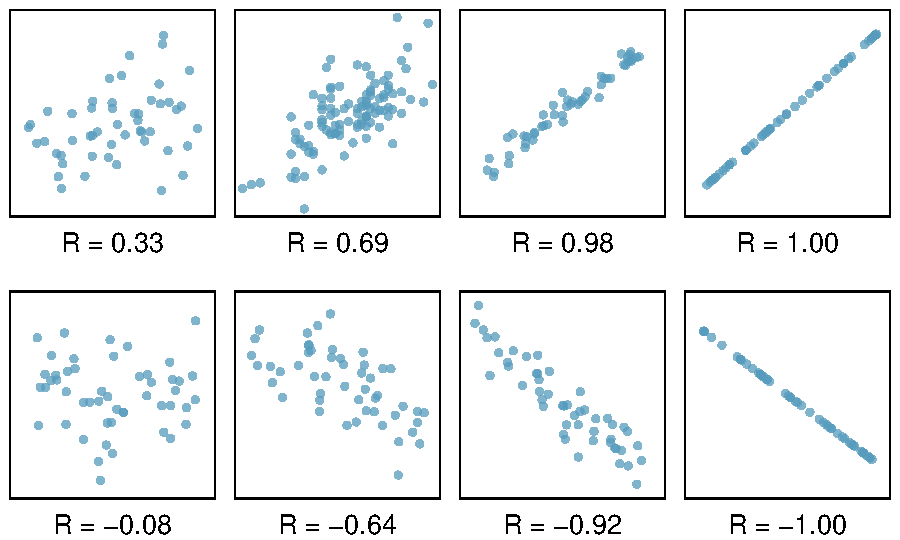
\includegraphics[width=0.95\textwidth]{07/figures/posNegCorPlots/posNegCorPlots}
   \caption{Sample scatterplots and their correlations. The first row shows variables with a positive relationship, represented by the trend up and to the right. The second row shows variables with a negative trend, where a large value in one variable is associated with a low value in the other.}
   \label{posNegCorPlots}
\end{figure}

The correlation is intended to quantify the strength of a linear trend. Nonlinear trends, even when strong, sometimes produce correlations that do not reflect the strength of the relationship; see three such examples in Figure~\ref{corForNonLinearPlots}.
\begin{figure}
   \centering
   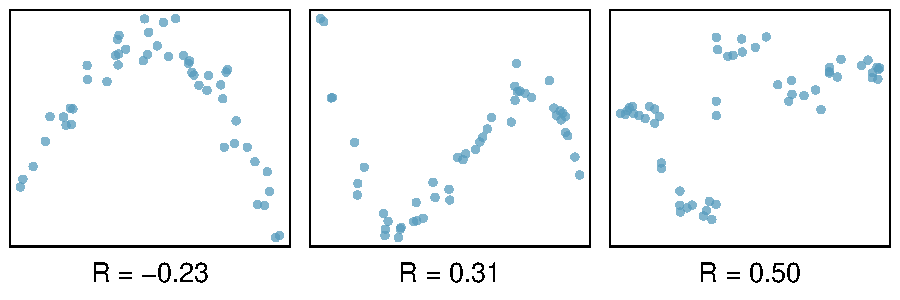
\includegraphics[width=0.96\textwidth]{07/figures/posNegCorPlots/corForNonLinearPlots}
   \caption{Sample scatterplots and their correlations. In each case, there is a strong relationship between the variables. However, the correlation is not very strong, and the relationship is not linear.}
   \label{corForNonLinearPlots}
\end{figure}

\begin{exercise}
While no straight line will fit any of the data sets in any of the scatterplots shown in Figure~\ref{corForNonLinearPlots}, try drawing nonlinear curves to each plot. Once you create a curve for each, describe what is important in your fit. Comment in the footnote\footnote{Possible explanation: The line should be close to most points and reflect overall trends in the data.}.
\end{exercise}

%%%%%%%%%%%%
\section{Fitting a line by least squares regression}
\label{fittingALineByLSR}

Fitting linear models by eye is (rightfully) open to criticism since it is based on an individual preference. In this section, we propose \emph{least squares regression} as a more rigorous approach.

This section will use data on SAT math scores and first year GPA from a random sample of students at a college\footnote{These data were collected by Educational Testing Service from an unnamed college. More information:\\https://www.dartmouth.edu/~chance/course/Syllabi/Princeton96/Class12.html}. A scatterplot of the data is shown in Figure~\ref{satGPAAllTwoLinesFitted} along with two linear fits. The lines follow a positive trend in the data; students who scored higher math SAT scores also tended to have higher GPAs after their first year in school.
\begin{figure}
\centering
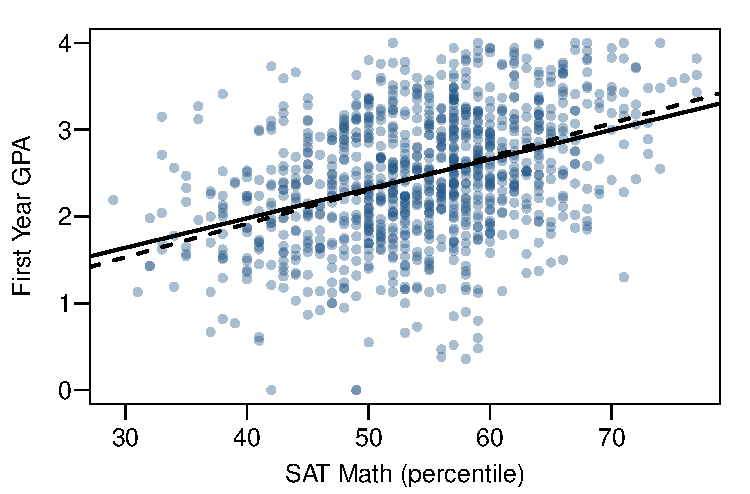
\includegraphics[width=0.7\textwidth]{07/figures/satGPA/satGPAAllTwoLinesFitted}
\caption{SAT math (percentile) and GPA scores for students after one year in college. Two lines are fit to the data, the solid line being the \emph{least squares line}.}
\label{satGPAAllTwoLinesFitted}
\end{figure}

\begin{exercise}
Is the correlation positive or negative? Answer in the footnote\footnote{Positive: because larger SAT scores are associated with higher GPAs, the correlation will be positive. Using a computer, the correlation can be computed: 0.387.}.
\end{exercise}

\subsection{An objective measure for finding the best line}

We begin by thinking about what we mean by ``best''. Mathematically, we want a line that has small residuals. Perhaps our criterion could minimize the sum of the residual magnitudes:
\begin{eqnarray}
|e_1| + |e_2| + \dots + |e_n|
\label{sumOfAbsoluteValueOfResiduals}
\end{eqnarray}
We could use a computer program to find a line that minimizes this criterion (the sum). This does result in a pretty good fit, which is shown as the dashed line in Figure~\ref{satGPAAllTwoLinesFitted}. However, a more common practice is to choose the line that minimizes the sum of the squared residuals:
\begin{eqnarray}
e_{1}^2 + e_{2}^2 + \dots e_{n}^2
\label{sumOfSquaresForResiduals}
\end{eqnarray}
The line that minimizes this \term{least squares criterion} is represented as the solid line in Figure~\ref{satGPAAllTwoLinesFitted}. This is commonly called the \term{least squares line}. Three possible reasons to choose Criterion~\eqref{sumOfSquaresForResiduals} over Criterion~\eqref{sumOfAbsoluteValueOfResiduals} are the following:
\begin{enumerate}
\item It is the most commonly used method.
\item Computing the line based on Criterion~\eqref{sumOfSquaresForResiduals} is much easier by hand and in most statistical software.
\item In many applications, a residual twice as large as another is more than twice as bad. For example, being off by 4 is usually more than twice as bad as being off by 2. Squaring the residuals accounts for this discrepancy.
\end{enumerate}
The first two reasons are largely for tradition and convenience, and the last reason explains why Criterion~\eqref{sumOfSquaresForResiduals} is typically most helpful\footnote{There are applications where Criterion~\eqref{sumOfAbsoluteValueOfResiduals} may be more useful, and there are plenty of other criteria we might consider. However, this book only applies the least squares criterion.}.

\subsection{Conditions for the least squares line}

When fitting a least squares line, we generally require
\begin{itemize}
\item \textbf{Linearity.} The data should show a linear trend. If there is a nonlinear trend (e.g. left panel of Figure~\ref{whatCanGoWrongWithLinearModel}), an advanced regression method from another book or later course should be applied.
\item \textbf{Nearly normal residuals.} Generally the residuals must be nearly normal.
When this condition is found to be unreasonable, it is usually because of outliers or concerns about influential points, which we  will discuss in greater depth in Section~\ref{typesOfOutliersInLinearRegression}. An example of non-normal residuals is shown in the center panel of Figure~\ref{whatCanGoWrongWithLinearModel}.
\item \textbf{Constant variability.} The variability of points around the least squares line remains roughly constant. An example of non-constant variability is shown in the right panel of Figure~\ref{whatCanGoWrongWithLinearModel}.
\end{itemize}
\begin{figure}
\centering
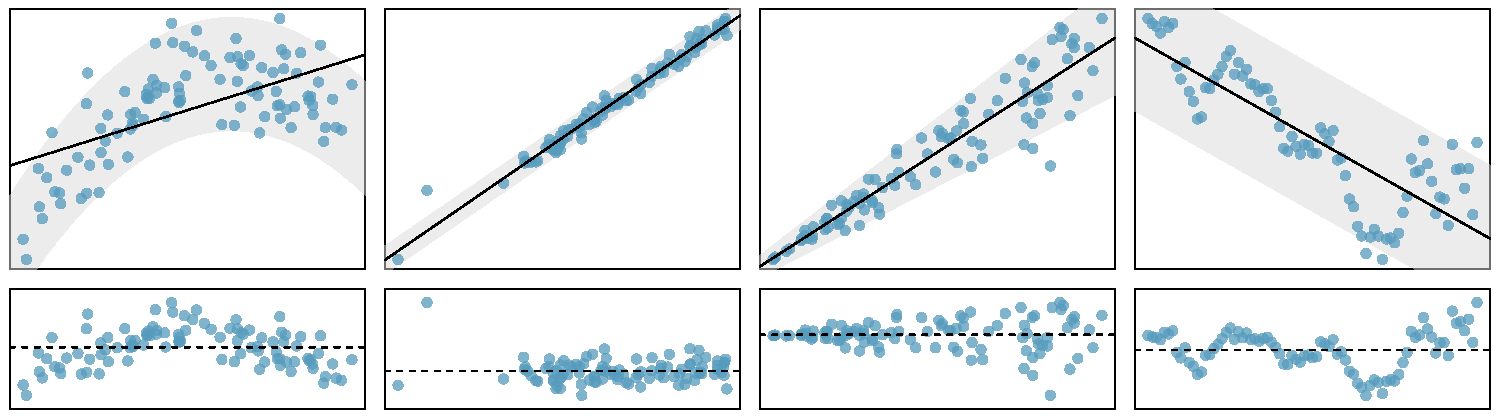
\includegraphics[width=122mm]{07/figures/whatCanGoWrongWithLinearModel/whatCanGoWrongWithLinearModel}
\caption{Three examples showing when the methods in this chapter are insufficient to apply to the data. In the left panel, a straight line does not fit the data. In the second panel, there are outliers; two points on the left are relatively distant from the rest of the data and one of these points is very far away from the line. In the third panel, the variability of the data around the line increases with larger values of $x$.}
\label{whatCanGoWrongWithLinearModel}
\end{figure}

\begin{exercise}
Should you have any concerns about applying least squares to the \var{satMath} and \var{GPA} data in Figure~\vref{satGPAAllTwoLinesFitted}? Answer in the footnote\footnote{The trend appears to be linear, the data fall around the line with no obvious outliers, and the variance is roughly constant. Least squares regression can be applied to these data.}.
\end{exercise}

\subsection{Finding the least squares line}
\label{findingTheLeastSquaresLineSection}

For the \var{satMath} and \var{GPA} data, we could write the equation as
\begin{eqnarray}
\widehat{GPA} = \beta_0 + \beta_1*satMath
\label{LSRLineForSATMathToPredictGPAStillWithParametersUnknown}
\end{eqnarray}
Here the equation is set up to predict \var{GPA} based on a student's \var{satMath} score, which would be useful to a college admissions office. These two values, $\beta_0$ and $\beta_1$, are the \emph{parameters} of the regression line.

Just like in Chapters~4-6, the parameters are estimated using observed data. In practice, this estimation is done using a computer in the same way that other estimates, like a sample mean, can be estimated using a computer or calculator. However, we can also find the parameter estimates by applying two properties of the least squares line: %\footnote{These properties follow from the mathematics that lie behind least squares regression. Deriving these properties is beyond the scope of this course.}:
\begin{itemize}
\item If $\bar{x}$ is the mean of the horizontal variable (from the data) and $\bar{y}$ is the mean of the vertical variable, then the point $(\bar{x}, \bar{y})$ is on the least squares line.
\item The slope of the least squares line is estimated by
\begin{eqnarray}
b_1 = \frac{s_y}{s_x} R
\label{slopeOfLSRLine}
\end{eqnarray}
where $R$ is the correlation between the two variables, and $s_x$ and $s_y$ are the sample standard deviations of the explanatory variable (variable on the horizontal axis) and response (variable on the vertical axis), respectively.
\end{itemize}
\marginpar[\raggedright\vspace{0.5mm}

$b_0, b_1$\vspace{0.5mm}\\\footnotesize Sample\\estimates\\ of $\beta_0$, $\beta_1$]{\raggedright\vspace{0.5mm}

$b_0, b_1$\vspace{0.5mm}\\\footnotesize Sample\\estimates\\ of $\beta_0$, $\beta_1$}We use $b_1$ to represent the point estimate of the parameter $\beta_1$, and we will similarly use $b_0$ to represent the sample point estimate for $\beta_0$.

\begin{exercise}
Table~\ref{summaryStatsOfSATGPAData} shows the sample means for the \var{satMath} and \var{GPA} variables: 54.395 and 2.468. Plot the point $(54.395, 2.468)$ on Figure~\vref{satGPAAllTwoLinesFitted} to verify it falls on the least squares line (the solid line).
\end{exercise}
\begin{table}[ht]
\centering
\begin{tabular}{l rr}
\hline
	&	\var{satMath} (``$x$'')	& \var{GPA} (``$y$'') \\
\hline
mean	& $\bar{x} = 54.395$		& $\bar{y} = 2.468$ \\
sd		& $s_x = 8.450$		& $s_y = 0.741$ \\
\hline
	& \multicolumn{2}{r}{correlation: $R=0.387$} \\
\hline
\end{tabular}
\caption{Summary statistics for the \var{satMath} and \var{GPA} data.}
\label{summaryStatsOfSATGPAData}
\end{table}

\begin{exercise} \label{findingTheSlopeOfTheLSRLineForSATMathAndGPA}
Using the summary statistics in Table~\ref{summaryStatsOfSATGPAData}, compute the slope for the regression line of GPA against SAT math percentiles. Answer in the footnote\footnote{Apply Equation~\eqref{slopeOfLSRLine} with the summary statistics from Table~\ref{summaryStatsOfSATGPAData} to compute the slope:
\begin{eqnarray*}
b_1 = \frac{s_y}{s_x} R = \frac{0.741}{8.450}0.387 = 0.03394
\end{eqnarray*}}.
\end{exercise}

You might recall from math class the \term{point-slope} form of a line (another common form is \emph{slope-intercept}). Given the slope of a line and a point on the line, $(x_0, y_0)$, the equation for the line can be written as
\begin{eqnarray}
y - y_0 = slope*(x - x_0)
\label{pointSlopeFormForALine}
\end{eqnarray}
A common exercise to become more familiar with foundations of least squares regression is to use basic summary statistics and point-slope form to produce the least squares line. 

\begin{tipBox}{\tipBoxTitle{Identifying the least squares line from summary statistics}
To identify the least squares line from summary statistics:
\begin{itemize}
\item Estimate the slope parameter, $b_1$, using Equation~(\ref{slopeOfLSRLine})
\item Noting that the point $(\bar{x}, \bar{y})$ is on the least squares line, use $x_0=\bar{x}$ and $y_0=\bar{y}$ along with the slope $b_1$ in the point-slope equation:
$$y - \bar{y} = b_1 (x - \bar{x}) $$
\item Simplify the equation.
\end{itemize}}
\end{tipBox}

\begin{example}{Using the point $(54.395, 2.468)$ from the sample means and the slope estimate $b_1 = 0.034$ from Exercise~\exer{findingTheSlopeOfTheLSRLineForSATMathAndGPA}, find the least-squares line for predicting \var{GPA} based on \var{satMath}.} \label{exampleToFindLSRLineOfSATGPAData}
Apply the point-slope equation using $(54.395, 2.468)$ and the slope, $b_1 = 0.03394$:
\begin{align*}
y - y_0     &= b_1 (x - x_0) \\
y - 2.468  &= 0.03394(x - 54.395)
\end{align*}
Expanding the right side and then adding 2.468 to each side, the equation simplifies:
$$ \widehat{GPA} = 0.622 + 0.03394 * satMath $$
Here we have replaced $y$ with $\widehat{GPA}$ and $x$ with $satMath$ to put the equation in context. This form matches the form of Equation~\eqref{LSRLineForSATMathToPredictGPAStillWithParametersUnknown}.
\end{example}

We mentioned earlier that a computer is usually used to compute the least squares line. A summary table based on some computer output is shown in Table~\ref{rOutputForSATGPALSRLine} for the \var{satMath} and \var{GPA} data. The first column of numbers provide estimates for ${b}_0$ and ${b}_1$, respectively. Compare these to the result from Example~\exam{exampleToFindLSRLineOfSATGPAData}.


%ZZQ Formatting
\pagebreak

\begin{table}[ht]
\centering
\begin{tabular}{l rrrr}
  \hline
 & Estimate & Std. Error & t value & Pr($>$$|$t$|$) \\ 
  \hline
(Intercept) & 0.6219 & 0.1408 & 4.42 & 0.0000 \\ 
 satMath & 0.0339 & 0.0026 & 13.26 & 0.0000 \\ 
   \hline
\end{tabular}
\caption{Summary of least squares fit for the SAT/GPA data. Compare the parameter estimates in the first column to the results of Example~\exam{exampleToFindLSRLineOfSATGPAData}.\vspace{-3mm}}
\label{rOutputForSATGPALSRLine}
\end{table}

\begin{example}{Examine the second, third, and fourth columns in Table~\ref{rOutputForSATGPALSRLine}. Can you guess what they represent?}
These columns help determine whether the estimates are significantly different from zero and to create a confidence interval for each parameter. The second column lists the standard errors of the estimates, the third column contains $t$ test statistics, and the fourth column lists p-values (2-sided test). We will describe the interpretation of these columns in greater detail in Section~\ref{inferenceForLinearRegression}.
\end{example}

\subsection{Interpreting regression line parameter estimates}

Interpreting parameters in a regression model is often one of the most important steps in the analysis.

\begin{example}{The slope and intercept estimates for the SAT-GPA data are 0.6219 and 0.0339. What do these numbers really mean?}
The intercept $b_0=0.6219$ describes the average GPA if a student was at the zeroth percentile score, if the linear relationship held all the way to $satMath=0$. This interpretation -- while perhaps interesting -- may not be very meaningful since there are no students enrolled at this college who are very close to the zeroth percentile.

Interpreting the slope parameter is often more realistic and helpful. For each additional SAT percentile score, we would expect a student to have an additional 0.0339 points in their first-year GPA on average. We must be cautious in this interpretation: while there is a real association, we cannot interpret a causal connection between the variables. That is, increasing a student's SAT score may not cause the student's GPA to increase.
\end{example}

\begin{termBox}{\tBoxTitle{Interpreting least squares estimate parameters}
The intercept describes the average outcome of $y$ if $x=0$ \emph{and} the linear model holds. The slope describes the estimated difference in the $y$ variable if the explanatory variable ($x$) for a case happened to be one unit larger.}
\end{termBox}

\subsection{Extrapolation is treacherous}

{\em\small When those blizzards hit the East Coast this winter, it proved to my satisfaction that global warming was a fraud. That snow was freezing cold. But in an alarming trend, temperatures this spring have risen. Consider this: On February $6^{th}$ it was 10 degrees. Today it hit almost 80. At this rate, by August it will be 220 degrees. So clearly folks the climate debate rages on.\vspace{0.5mm}}

\noindent\hspace{\textwidth}\hspace{-40mm}Stephen Colbert

\noindent\hspace{\textwidth}\hspace{-40mm}April 6th, 2010 \footnote{http://www.colbertnation.com/the-colbert-report-videos/269929/} \\

Linear models are used to approximate the relationship between two variables. However, these models have real limitations. Linear regression is simply a modeling framework. The truth is almost always much more complex than our simple line. For example, we do not know how the data outside of our limited window will behave.

SAT math scores were used to predict freshman GPA in Section~\ref{findingTheLeastSquaresLineSection}. We could also use the overall percentile as a predictor in place of just the math score:
\begin{align*}
\widehat{GPA} = 0.0019 + 0.0477*satTotal
\end{align*}
These data are shown in Figure~\ref{overallSATGPADataWithLSRLine}. The linear model in this case was built for observations between the $26^{th}$ and the $72^{nd}$ percentiles. The data meet all conditions necessary for the least squares regression line, so could the model safely be applied to students at the $90^{th}$ percentile?
\begin{figure}
\centering
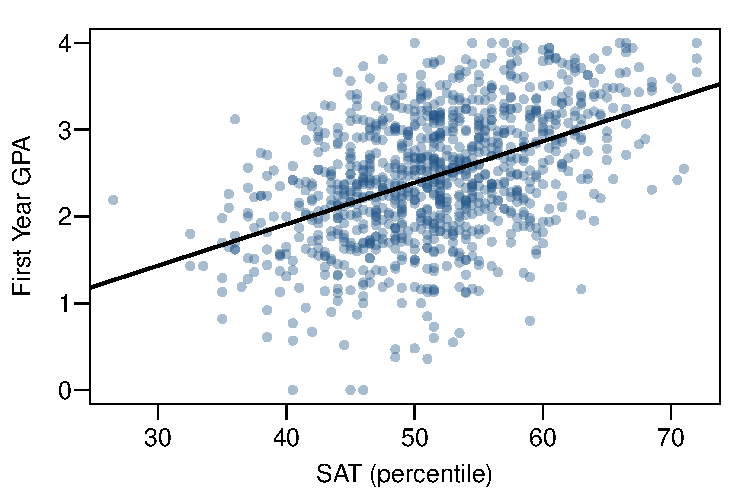
\includegraphics[width=0.75\textwidth]{07/figures/satGPA/overallSATGPADataWithLSRLine}
\caption{A scatterplot of GPA scores versus overall SAT percentile. The least squares regression line is shown.}
\label{overallSATGPADataWithLSRLine}
\end{figure}

\begin{example}{Use the model $\widehat{GPA} = 0.0019 + 0.0477*satTotal$ to estimate the GPA of a student who is at the $90^{th}$ percentile.}
To predict the GPA for a person with an SAT percentile of 90, we plug 90 into the regression equation:
\begin{align*}
0.0019 + 0.0477*satTotal  = 0.0019 + 0.0477*90 = 4.29
\end{align*}
The model predicts a GPA score of 4.29. GPAs only go up to 4.0 (!).
\end{example}

Applying a model estimate to values outside of the realm of the original data is called \term{extrapolation}. Generally, a linear model is only an approximation of the real relationship between two variables. If we extrapolate, we are making an unreliable bet that the approximate linear relationship will be valid in places where it has not been analyzed.

\subsection{Using $R^2$ to describe the strength of a fit}

We evaluated the strength of the linear relationship between two variables earlier using correlation, $R$. However, it is more common to explain the strength of a linear fit using $R^2$, called \term{R-squared}. If we are given a linear model, we would like to describe how closely the data cluster around the linear fit.

The $R^2$ of a linear model describes the amount of variation in the response that is explained by the least squares line. For example, consider the SAT-GPA data, shown in Figure~\ref{overallSATGPADataWithLSRLine}. The variance of the response variable, \var{GPA}, is $s_{_{GPA}}^2=0.549$. However, if we apply our least squares line, then this model reduces our uncertainty in predicting GPA using a student's SAT score. The variability in the residuals describes how much variation remains after using the model: $s_{_{RES}}^2 = 0.433$. In short, there was a reduction of
$$\frac{s_{_{GPA}}^2 - s_{_{RES}}^2}{s_{_{GPA}}^2}
	= \frac{0.549 - 0.433}{0.549} = \frac{0.116}{0.549}
	= 0.21$$
or about  21\% in the data's variation by using information about the SAT scores via a linear model. This corresponds exactly to the R-squared value:
\begin{align*}
R &= 0.46 &R^2 &= 0.21
\end{align*}

\begin{exercise}
If a linear model has a very strong negative relationship with a correlation of -0.97, how much of the variation in the response is explained by the explanatory variable? Answer in the footnote\footnote{About $R^2 = (-0.97)^2 = 0.94$ or 94\% of the variation is explained by the linear model.}.
\end{exercise}

%%%%%%%%%%%%%
\section{Types of outliers in linear regression}
\label{typesOfOutliersInLinearRegression}

In this section, we identify (loose) criteria for which outliers are important and influential.

Outliers in regression are observations that fall far from the ``cloud'' of points. These points are especially important because they can have a strong influence on the least squares line. 

\begin{exercise} \label{outlierPlotsExercise}
There are six plots shown in Figure~\ref{outlierPlots} along with the least squares line and residual plots. For each scatterplot and residual plot pair, identify any obvious outliers and note how you think they influence the least squares line. Recall that an outlier is any point that doesn't appear to belong with the vast majority of the other points. Answer in the footnote\footnote{Across the top, then across the bottom: (1) There is one outlier far from the other points, though it only appears to slightly influence the line. (2) One outlier on the right, though it is quite close to the least squares line, which suggests it wasn't very influential. (3) One point is far away from the cloud, and this outlier appears to pull the least squares line up on the right; examine how the line around the primary cloud doesn't appear to fit very well. (4) There is a primary cloud and then a small secondary cloud of four outliers. The secondary cloud appears to be influencing the line somewhat strongly, making the least square line fit poorly almost everywhere. There might be an interesting explanation for the dual clouds, which is something that could be investigated. (5) there is no obvious trend in the main cloud of points and the outlier on the right appears to largely control the slope of the least squares line. (6) There is one outlier far from the cloud, however, it falls quite close to the least squares line and does not appear to be very influential.}.
\end{exercise}
\begin{figure}
\centering
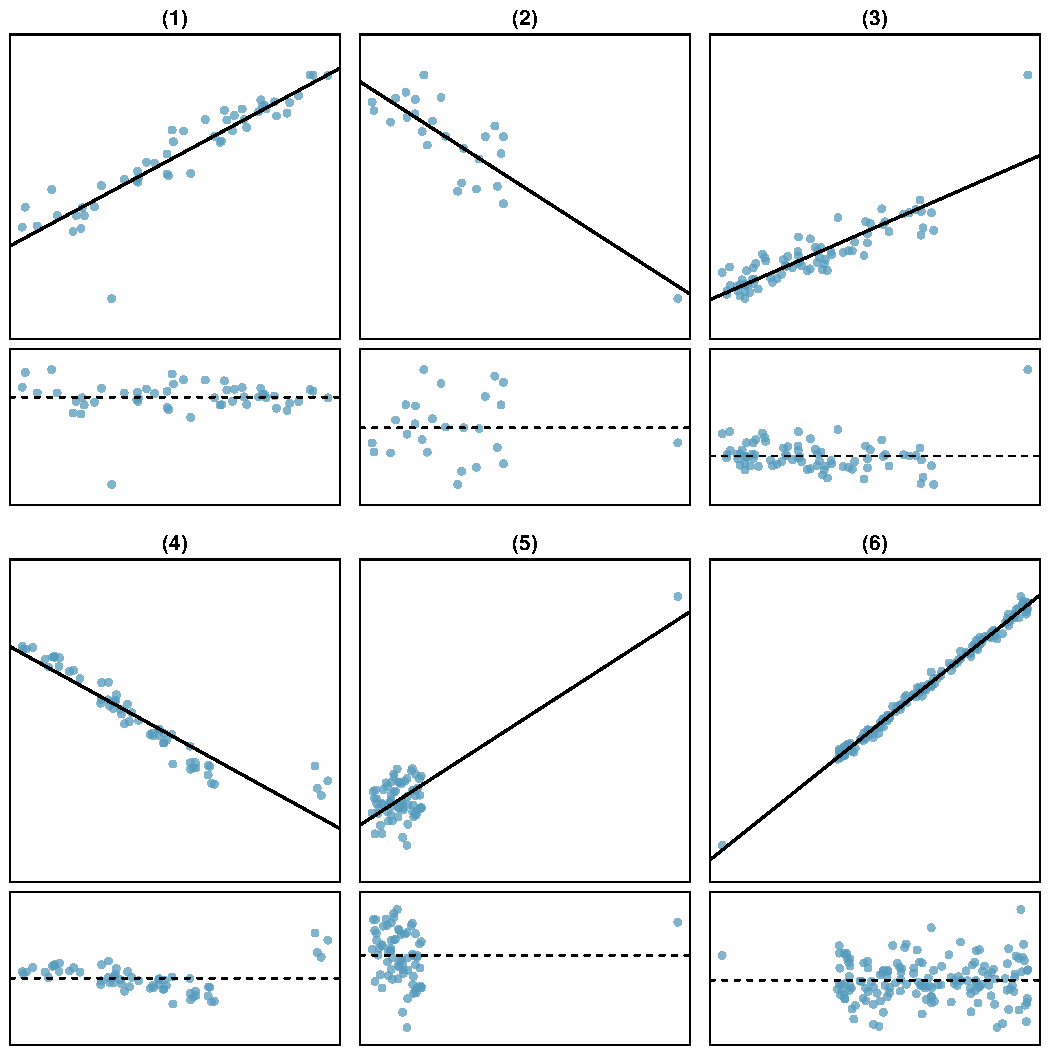
\includegraphics[width=0.99\textwidth]{07/figures/outlierPlots/outlierPlots}
\caption{Six plots, each with a least squares line and residual plot. All data sets have at least one outlier.}
\label{outlierPlots}
\end{figure}

Examine the residual plots in Figure~\ref{outlierPlots}. You will probably find that there is some trend in the main clouds of (3) and (4). In these cases, the outlier influenced the slope of the least squares line. In (5), data with no clear trend were assigned a line with a large trend simply due to one outlier (!).
 
 \begin{termBox}{\tBoxTitle{Leverage}
Points that fall, horizontally, away from the center of the cloud tend to pull harder on the line, so we call them points with \term{high leverage}.}
\end{termBox}

Points that fall horizontally far from the line are points of high leverage; these points can strongly influence the slope of the least squares line. If one of these high leverage points does appear to actually invoke its influence on the slope of the line -- as in cases (3), (4), and (5) of Exercise~\exer{outlierPlotsExercise} -- then we call it an \term{influential point}. Usually we can say a point is influential if, had we fit the line without it, the influential point would have been unusually far from the least squares line.

It is tempting to remove outliers. Don't do this without very good reason. Models that ignore exceptional (and interesting) cases often perform poorly. For instance, if a financial firm ignored the largest market swings -- the ``outliers'' --  they would soon go bankrupt by making poorly thought-out investments.

\begin{caution}{Don't ignore outliers when fitting a final model}
{If there are outliers in the data, they should not be removed or ignored without good reason. Whatever final model is fit to the data would not be very helpful if it ignores the most exceptional cases.}
\end{caution}

%%%%%%%%%
\section{Inference for linear regression}
\label{inferenceForLinearRegression}

In this section we discuss uncertainty in the estimates of the slope and y-intercept for a regression line. Just as we identified standard errors for point estimates in previous chapters, we first discuss standard errors for these new estimates. However, in the case of regression, we will identify standard errors using statistical software.

\subsection{Midterm elections and unemployment}

Elections for members of the United States House of Representatives occur every two years, coinciding every four years with the U.S. Presidential election. The set of House elections occurring during the middle of a Presidential term are called \indexthis{midterm elections}{midterm election}, and are thought to be closely linked with unemployment. In America's two-party system, one political theory suggests the higher the unemployment rate, the worse the President's party will do in the midterm elections.

To assess the validity of this claim, we can compile historical data and look for a connection. We consider every midterm election from 1898 to 2010, with the exception of those elections during the Great Depression. Figure~\ref{unemploymentAndChangeInHouse} shows these data and the least-squares regression line:
\begin{align*}
&\text{\% change in House seats for President's party}  \\
&\qquad\qquad= -2.94 - 1.08*\text{(unemployment rate)}
\end{align*}
We consider the percent change in the number of seats of the President's party (e.g. percent change in the number of seats for Democrats in 2010) against the unemployment rate.
\begin{figure}
\centering
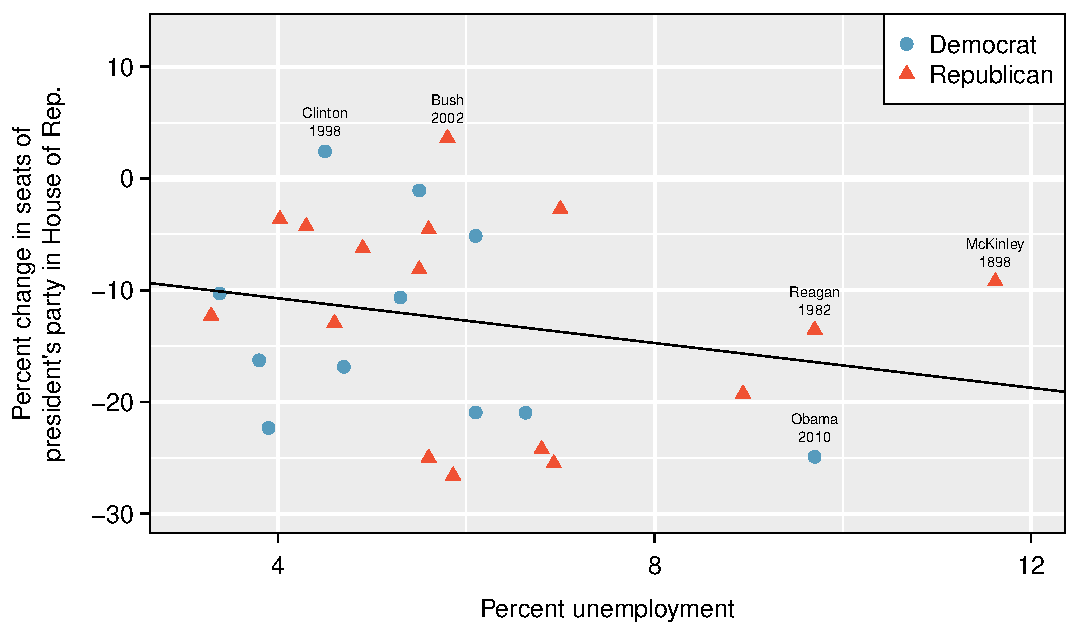
\includegraphics[width=0.87\textwidth]{07/figures/unemploymentAndChangeInHouse/unemploymentAndChangeInHouse}
\caption{The percent change in House seats for the President's party in each election from 1898 to 2010 plotted against the unemployment rate. The two points for the Great Depression have been removed, and a least squares regression line has been fit to the data.}
\label{unemploymentAndChangeInHouse}
\end{figure}

\begin{exercise}
The data for the Great Depression (1934 and 1938) were removed because the unemployment rate was 21\% and 18\%, respectively. Do you agree that they should be removed for this investigation? Why or why not? Two considerations in the footnote\footnote{Each of these points would have very high leverage on any least-squares regression line, and years with such high unemployment may not help us understand what would happen in other years where the unemployment is only modestly high. On the other hand, these are exceptional cases, and we would be discarding important information if we exclude them from a final analysis.}.
\end{exercise}

There is a negative slope in the line shown in Figure~\ref{unemploymentAndChangeInHouse}. However, this slope (and the y-intercept) are only estimates of the parameter values. We might wonder, is this convincing evidence that the ``true'' linear model has a negative slope? That is, do the data provide strong evidence that the political theory is accurate? We can frame this investigation into a one-sided statistical hypothesis test:
\begin{itemize}
\item[$H_0$:] $\beta_1 = 0$. The true linear model has slope zero.
\item[$H_A$:] $\beta_1 < 0$. The true linear model has a negative slope. That is, the higher the unemployment, the greater the losses for the President's party in the House of Representatives.
\end{itemize}
We would reject $H_0$ in favor of $H_A$ if the data provide strong evidence that the true slope parameter is less than zero. To assess the hypothesis test, we identify a standard error for the estimate, compute an appropriate test statistic, and identify the p-value.

\subsection{Understanding regression output from software}
\label{testStatisticForTheSlope}

Just like other point estimates we have seen before, we can compute a standard error for $b_1$ and a test statistic. We will generally label the test statistic using a $T$, since it follows the $t$ distribution.

We will rely on statistical software to compute the standard error and leave the derivation to a second or third statistics course. Table~\ref{midtermElectionUnemploymentRRegressionOutput} shows software output for the least squares regression line in Figure~\ref{unemploymentAndChangeInHouse}. The row labeled \emph{unemp} represents the information for the slope, which is the coefficient of the unemployment variable.
\begin{table}[ht]
\centering
\begin{tabular}{rrrrr}
  \hline
 & Estimate & Std. Error & t value & Pr($>$$|$t$|$) \\ 
  \hline
(Intercept) & -2.9417 & 9.0851 & -0.32 & 0.7488 \\ 
  unemp & -1.0805 & 1.4513 & -0.74 & 0.4635 \\ 
   \hline
   \multicolumn{5}{r}{$df=25$} \\
\end{tabular}
\caption{Output from statistical software for the regression line modeling the midterm election losses for the President's party as a response to unemployment.}
\label{midtermElectionUnemploymentRRegressionOutput}
\end{table}

\begin{example}{There are two rows in Table~\ref{midtermElectionUnemploymentRRegressionOutput}: one for the y-intercept estimate and one for the slope estimate. What do the first and second columns represent?}
The entries in the first column represent the least squares estimate, and the values in the second column correspond to the standard errors of each estimate.
\end{example}

We previously used a $t$ test statistic for hypothesis testing on small (or large!) samples. Regression is very similar. In the hypotheses we consider, the null value for the slope is 0, so we can compute the test statistic using the T (or Z) score formula:
\begin{align*}
T = \frac{\text{estimate} - \text{null value}}{\text{SE}} = \frac{-1.0808 - 0}{1.4513} = -0.74
\end{align*}
We can look for the one-sided p-value -- shown in Figure~\ref{oneSidedTailForMidtermUnemploymentHT} -- using the probability table for the $t$ distribution in Appendix~\ref{tDistributionTable} on page~\pageref{tDistributionTable}.
\begin{figure}
\centering
\includegraphics[width=0.8\textwidth]{07/figures/oneSidedTailForMidtermUnemploymentHT/oneSidedTailForMidtermUnemploymentHT}
\caption{The distribution shown here is the sampling distribution for $b_1$, if the null hypothesis was true. The shaded tail represents the p-value for the hypothesis test evaluating whether there is convincing evidence that higher unemployment corresponds to a greater loss of House seats for the President's party during a midterm election.}
\label{oneSidedTailForMidtermUnemploymentHT}
\end{figure}

%ZZQ Formatting
\pagebreak

\begin{example}{Table~\ref{midtermElectionUnemploymentRRegressionOutput} offers the degrees of freedom for the test statistic $T$: $df=25$. Identify the p-value for the hypothesis test.}
Looking in the 25 degrees of freedom row in Appendix~\ref{tDistributionTable}, we see that the absolute value of the test statistic is smaller than any value listed, which means the tail area and therefore also the p-value is larger than 0.100 (one tail!). Because the p-value is so large, we fail to reject the null hypothesis. That is, the data do not provide convincing evidence that a higher unemployment rate tends to correspond to larger losses for the President's party in the House of Representatives in midterm elections.
\end{example}

We could have identified the $t$ test statistic from the software output in Table~\ref{midtermElectionUnemploymentRRegressionOutput}, shown in the second row (unemp) and third column under (t value). The entry in the second row and last column in Table~\ref{midtermElectionUnemploymentRRegressionOutput} represents the p-value for the \emph{two-sided} hypothesis test where the null value is zero. Under close examination, we can see a null hypothesis of 0 was also used to compute the p-value in the \emph{(Intercept)} row. However, we are more often interested in evaluating the significance of the slope since the slope represents a connection between the two variables while the intercept represents an estimate of the average outcome if the x-value was zero.

\begin{termBox}{\tBoxTitle{Inference for regression}
We usually rely on statistical software to identify point estimates and standard errors for parameters of a regression line. After verifying conditions hold for fitting a line, we can use the methods learned in Section~6.1 for the $t$ distribution to create confidence intervals for regression parameters or to evaluate hypothesis tests.}
\end{termBox}

\begin{caution}{Don't carelessly use the p-value from regression output}{The last column in regression output is often used to list p-values for one particular hypothesis: a two-sided test where the null value is zero. If your test is one-sided and the point estimate is in the direction of $H_A$, then you can halve the software's p-value to get the one-tail area. If neither of these scenarios match your hypothesis test, be cautious about using the software output to obtain the p-value.}
\end{caution}

\begin{example}{Examine Figure~\ref{overallSATGPADataWithLSRLine} on page~\pageref{overallSATGPADataWithLSRLine}, which relates freshman GPA and SAT scores. How sure are you that the slope is statistically significantly different from zero? That is, do you think a formal hypothesis test would reject the claim that the true slope of the line should be zero? Why or why not?} \label{overallSATGPAInformalAssessmentOfRegressionLineSlope}
While the relationship between the variables is not perfect, it is difficult to deny that there is some increasing trend in the data. This suggests the hypothesis test will reject the null claim that the slope is zero.
\end{example}

\begin{exercise}
Table~\ref{rOutputForSATGPALSRLineInInferenceSection} shows statistical software output from fitting the least squares regression line shown in Figure~\ref{overallSATGPADataWithLSRLine}. Use this output to formally evaluate the following hypotheses. $H_0$: The true coefficient for \var{satTotal} is zero. $H_A$: The true coefficient for \var{satTotal} is not zero. Answer in the footnote\footnote{We look in the second row corresponding to the \var{satTotal} variable. We see the point estimate of the slope of the line is 0.0477, the standard error of this estimate is 0.0029, and the $t$ test statistic is 16.38. The p-value corresponds exactly to the two-sided test we are interested in: 0.0000. This output doesn't mean the p-value is exactly zero, only that when rounded to four decimal places it is zero. That is, the p-value is so small that we can reject the null hypothesis and conclude that GPA and SAT scores are positively correlated and the true slope parameter is indeed greater than 0, just as we believed in Example~\ref{overallSATGPAInformalAssessmentOfRegressionLineSlope}.}.
\end{exercise}
\begin{table}[ht]
\centering
\begin{tabular}{rrrrr}
  \hline
 & Estimate & Std. Error & t value & Pr($>$$|$t$|$) \\ 
  \hline
(Intercept) & 0.0019 & 0.1520 & 0.01 & 0.9899 \\ 
satTotal & 0.0477 & 0.0029 & 16.38 & 0.0000 \\ 
   \hline
\end{tabular}
\caption{Summary of least squares fit for the SAT/GPA data.}
\label{rOutputForSATGPALSRLineInInferenceSection}
\end{table}

\begin{tipBox}{\tipBoxTitle{Always check assumptions}
If conditions for fitting the regression line do not hold, then the methods presented here should not be applied. The standard error or distribution assumption of the point estimate -- assumed to be normal when applying the $t$ test statistic -- may not be valid.}
\end{tipBox}

\subsection{An alternative test statistic}

We considered the $t$ test statistic as a way to evaluate the strength of evidence for a hypothesis test in Section~\ref{testStatisticForTheSlope}. However, we could focus on $R^2$. Recall that $R^2$ described the proportion of variability in the response variable ($y$) explained by the explanatory variable ($x$). If this proportion is large, then this suggests a linear relationship exists between the variables. If this proportion is small, then the evidence provided by the data may not be convincing.

This concept -- considering the amount of variability in the response variable explained by the explanatory variable -- is a key component in some statistical techniques. A method called \term{analysis of variance (ANOVA)} relies on this general principle and is a common topic in statistics. The method states that if enough variability is explained away by the explanatory variable, then we would conclude the variables are connected. On the other hand, we might not be convinced if only a little variability is explained. We will discuss this method further in Section~\ref{anovaAndRegrWithCategoricalVariables}.


%\section{Beyond linear fits}
%This will be limited and will largely reference other books for further information.
%\subsection{Transformations on the response}
%\subsection{Regressing on many variables}
%\subsection{Non-linear fits}
%\label{nonLinearFits}

%\section{Diagnostics}

%Fitting a linear model to a data set is appropriate under certain conditions. It is important to verify that these conditions are reasonably met based on the data, just like how conditions were checked in Chapters~4, 5, and 6 %ZZQ \ref{}, \ref{}, \ref{}
%for inference techniques. We really need only check two conditions:
%\begin{enumerate}
%\item \textbf{Linearity.} Do the points follow a straight line?
%\item \textbf{Normality of residuals.} Are the residuals nearly normal?
%\end{enumerate}
%The first condition may be checked by examining a residual plot. Figure~\ref{} shows three plots, each with a residual 

%\subsection{Potential problems}
%\subsection{Checking the fit}

